\subsection{Outlier Analysis}

To understand the limitations of our computational approach, we analyzed the 59 molecules (15.6\% of the dataset) with prediction errors exceeding 0.3~eV. Figure~\ref{fig:SI_outlier_analysis} shows the distribution of these outliers and their characteristic descriptors.

\begin{figure}[!ht]
    \centering
    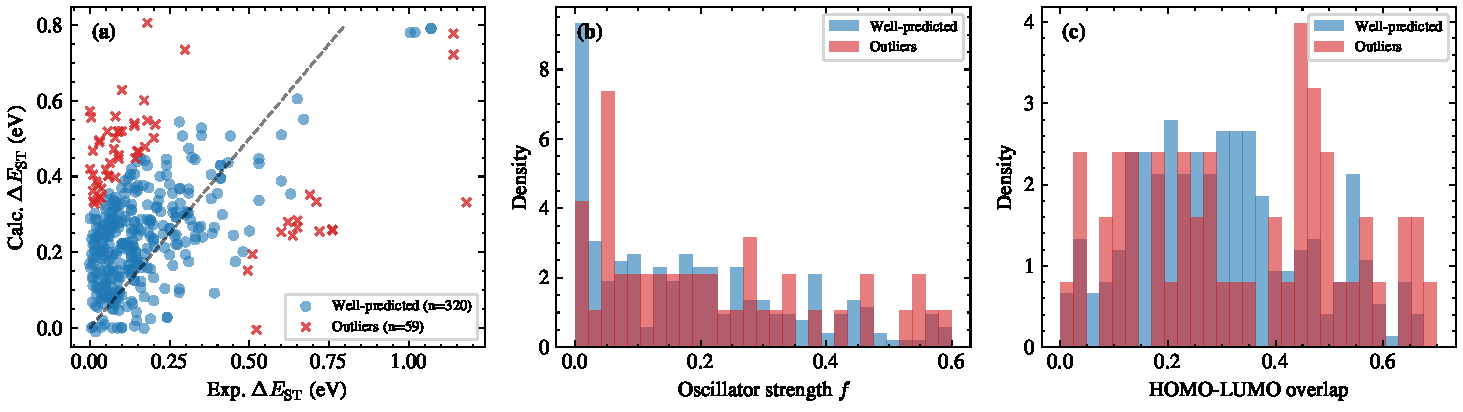
\includegraphics[width=\textwidth]{Figures/SI_outlier_analysis.pdf}
    \caption{Outlier analysis of the 379-molecule validation set. (a) Scatter plot highlighting outliers (red crosses, $|$error$|$ > 0.3~eV) versus 
well-predicted molecules (blue circles). (b) Distribution of oscillator strength $f$ for outliers and well-predicted molecules. (c) Distribution of HOMO-LUMO 
overlap for both groups. Outliers show systematically higher overlap values, indicating stronger charge-transfer character.}
    \label{fig:SI_outlier_analysis}
\end{figure}

\subsubsection{Error Patterns}

The outliers exhibit two distinct error patterns:
\begin{itemize}
    \item \textbf{Overestimation} (Calc $>$ Exp): 43 molecules (72.9\% of outliers), predominantly with very small experimental $\Delta E_{\mathrm{ST}}$ values 
($<$0.1~eV). The mean experimental value for this group is 0.04~eV, while calculations predict 0.41~eV, suggesting systematic overestimation for near-zero 
singlet-triplet gaps.
    
    \item \textbf{Underestimation} (Calc $<$ Exp): 16 molecules (27.1\% of outliers), primarily with large experimental $\Delta E_{\mathrm{ST}}$ values 
($>$0.5~eV). The mean experimental value is 0.72~eV versus calculated 0.32~eV, indicating difficulty in predicting molecules with large singlet-triplet 
splittings.
\end{itemize}

\subsubsection{Descriptor Analysis}

Outliers show distinct characteristics compared to well-predicted molecules:

\begin{itemize}
    \item \textbf{HOMO-LUMO overlap}: Outliers exhibit significantly higher overlap (0.394 $\pm$ 0.238) compared to well-predicted molecules (0.312 $\pm$ 
0.177). High overlap ($>$0.5) is present in 28.8\% of outliers versus only 13.4\% of well-predicted molecules, suggesting that strong orbital delocalization 
challenges the computational approach.
    
    \item \textbf{Oscillator strength}: Outliers show slightly elevated $f$ values (0.409 $\pm$ 0.447) compared to well-predicted molecules (0.366 $\pm$ 0.432), 
with 15.3\% having $f > 0.8$ indicating strong $\pi$-$\pi^*$ character.
    
    \item \textbf{Experimental range}: Nearly half of outliers (49.2\%) have experimental $\Delta E_{\mathrm{ST}} < 0.1$~eV, representing the challenging regime 
where thermal energy ($k_{\mathrm{B}}T \approx 0.026$~eV at 300~K) becomes comparable to the singlet-triplet gap.
\end{itemize}

\subsubsection{Architecture-Specific Patterns}

Outliers are not uniformly distributed across molecular architectures:

\begin{itemize}
    \item \textbf{1D-0A} (15 outliers, 25.4\%): Single-donor architectures show moderate systematic overestimation (mean error = +0.085~eV), with relatively low 
HOMO-LUMO overlap (0.343).
    
    \item \textbf{Unknown} (14 outliers, 23.7\%): Molecules with unclassified architectures exhibit the largest systematic overestimation (mean error = 
+0.237~eV) and highest overlap (0.479), suggesting complex electronic structures not captured by standard D-A classifications.
    
    \item \textbf{Multi-D/A} (14 outliers, 23.7\%): Complex multi-component systems show significant overestimation (mean error = +0.222~eV) despite low 
oscillator strength (0.197), indicating challenges in treating multiple charge-transfer pathways.
    
    \item \textbf{2D-0A} (10 outliers, 16.9\%): Dual-donor architectures display consistent overestimation (mean error = +0.211~eV) with moderate descriptors.
\end{itemize}

\subsubsection{Extreme Cases}

Table~\ref{tab:SI_extreme_outliers} lists the most challenging predictions. The worst case (IQ-Se) shows an underestimation of 0.85~eV for a molecule with 
experimental $\Delta E_{\mathrm{ST}} = 1.18$~eV, far outside the typical TADF range. Conversely, molecules like 3ai and PS-BZ-DMAC with near-zero experimental 
gaps are overestimated by $>$0.5~eV, likely due to environmental effects (solvent, solid-state packing) not captured in gas-phase calculations.

\begin{table}[!ht]
\centering
\caption{Top 10 most challenging predictions from the 379-molecule validation set.}
\label{tab:SI_extreme_outliers}
\small
\begin{tabular}{llcccccc}
\hline
Molecule & Architecture & Exp & Calc & Error & $f$ & Overlap \\
         &              & (eV) & (eV) & (eV) &     &         \\
\hline
IQ-Se & Multi-D/A & 1.180 & 0.332 & $-$0.848 & 0.077 & 0.559 \\
3ai & 1D-0A & 0.180 & 0.806 & +0.626 & 0.797 & 0.397 \\
OXD-7 & Unknown & 0.000 & 0.573 & +0.573 & 2.008 & 0.235 \\
PS-BZ-DMAC & 1D-0A & 0.004 & 0.556 & +0.551 & 1.150 & 0.444 \\
TPSi-F & Unknown & 0.100 & 0.629 & +0.529 & 0.343 & 0.846 \\
TXO-P-Si & Unknown & 0.522 & $-$0.005 & $-$0.528 & 0.000 & 0.079 \\
mTPA–PPI & 1D-0A & 0.760 & 0.258 & $-$0.502 & 0.535 & 0.250 \\
mTPA-PPI & 1D-0A & 0.760 & 0.260 & $-$0.500 & 0.556 & 0.251 \\
4-Ac & 1D-0A & 0.080 & 0.559 & +0.479 & 0.624 & 0.702 \\
SPBP-DPAC & 1D-0A & 0.030 & 0.496 & +0.466 & 0.857 & 0.486 \\
\hline
\end{tabular}
\end{table}

\subsubsection{Implications}

This analysis reveals that the computational approach performs best for molecules with:
\begin{itemize}
    \item Moderate $\Delta E_{\mathrm{ST}}$ values (0.1--0.5~eV)
    \item Low-to-moderate HOMO-LUMO overlap ($<$0.5)
    \item Well-defined D-A architectures
\end{itemize}

Conversely, predictions are less reliable for molecules with near-zero experimental gaps, high orbital overlap, or complex multi-component architectures. These limitations likely stem from the gas-phase approximation, which neglects environmental effects (solvent stabilization, solid-state packing) that can significantly modulate singlet-triplet gaps in real TADF systems.
